\chapter{Bayesian periodization of postembryonic CMZ activity}
\label{chap:CMZ}

\section{Preliminaries: Calculation of Bayesian evidence supports independent Log-Normal modelling of CMZ parameters}
To take up the question of how CMZ RPC activity evolves over time, we have collected observations of a variety of CMZ and retinal parameters derived from histological studies of cryosections of zebrafish eyes harvested over the first year of the animal's life. We wish to extract as much information as possible about the structure and time-evolution of the CMZ population as a whole, in order to know how to best model its constituent RPCs. The initial approach here will be to estimate parameters of the whole-eye CMZ from sample cryosections, and to use these estimates as the dataset which will inform our selection of appropriate models.

While it remains common to assume that population census data are Normally distributed, and so simply to calculate means and standard deviations as the statistical representation of the underlying population, it has been known for decades \cite{Heath1967} that Log-Normal distributions are usually better models of the outcomes produced by additive processes with small, variable steps (like population sizes or income distributions). We therefore start with the selection of appropriate models for the CMZ- and retina-level population measurements critical to the inferences that follow.

As a first pass at this question, we calculate the likelihood ratio for the hypothesis that the parameter measurements, and the calculated quantities derived from them, are Log-Normally distributed against the the one that they are simply Normally distributed. These results are displayed in Table \ref{PLHRtable}.

\begin{table}[!ht]
    \centering
    \caption{
    {\bf Likelihood ratio comparison between Normal and Log-Normal models of retinal population parameters}}
    \begin{tabular}{|l|l|l|l|}
    \hline
    {\bf Parameter} & {\bf $\mathcal{N}$ logLH} & {\bf Log-$\mathcal{N}$ logLH} & {\bf logLR} \\ \hline
    Sectional PCNA+ve & -285.611 & {\bf -283.214} & 2.397\\ \hline
    Lens diameter & {\bf -203.102} & -203.854 & -0.752\\ \hline
    CMZ annular pop.($\dagger$)  & -484.768 & {\bf -482.733} & 2.035\\ \hline
    RPE length & {\bf -368.232} & -368.609 & -0.377\\ \hline
    CR thickness ($\dagger$) & {\bf -240.858} & -241.032 & -0.174\\ \hline
    CR volume ($\dagger$) & -1091.615 & {\bf -1091.146} & 0.469\\ \hline
    \end{tabular}
    \begin{flushleft} $\mathcal{N}$: Normal distribution. logLH: logarithm of p(D|M), the likelihood of the data given the model. logLR: logarithm of the likelihood ratio; positive ratios in favour of the log-$\mathcal{N}$ model. Largest likelihoods are bolded. $\dagger$: Calculated quantities. Sectional PCNA+ve: population of PCNA-positive CMZ RPCs per 14$\mu$m cryosection. CMZ annular pop: population of annular CMZ. RPE: retinal pigmented epithelium. CR: cellular retina.
    \end{flushleft}
    \label{PLHRtable}
\end{table}

These results suggest that the organism-level population distribution of eye-level CMZ population counts, as assayed by PCNA immunostaining, is better modelled Log-Normally than Normally. This is true whether we test the primary per-section count meaurements, or the estimated whole-annulus population, calculated as described in \autoref{sec:lenspopest}, even though this quantity is calculated using the Normally-distributed lens diameter\footnote{The apparent superiority of the Normal model for lens diameter may be due to the paucity of data at later time points; as described in INSERT METHODS AUTOREF, lenses are difficult to retain in this histological context.}. The most likely Log-Normal representations of the CMZ populations are about two orders of magnitude more likely than the Normal alternative. Additionally, although Normal models are slightly favoured for describing the population-level distributions of RPE length and cellular retina thickness, the derived cellular retina volume quantity is better modeled by a Log-Normal distribution. As the two calculated quantities will be the primary ones used in our inferences about population-level CMZ dynamics, we are most concerned with these measures; at this point, the Log-Normal distribution looks to be more informative for both.

We have emphasized the danger of relying overmuch on the parameterisation of single most-likely model fits in \autoref{chap:SMMEoutro}, which is what the simple likelihood ratios above represent: the joint likelihood of the maximum a posteriori distribution fitted to the measurements taken from each age cohort. Since the choice of model describing the estimated annular population and retinal volume is critical to the success of later inferences, we used Galilean Monte Carlo-Nested Sampling (GMC-NS) to estimate the Bayesian evidence (the marginal probability of the data over all model parameterisations) for these hypotheses. Although it is very unlikely that GMC-NS will result in conclusions from the likelihood ratio, this simple test serves to prove the function of the \path{GMC_NS.jl} package, and demonstrate the inferential logic. Evidence estimates and ratios are presented in Table \ref{PZRtable}.

\begin{table}[!ht]
    \centering
    \caption{
    {\bf Evidence favours Log-Normal models of retinal population parameters}}
    \begin{tabular}{|l|l|l|l|l|}
    \hline
    {\bf Parameter} & {\bf $\mathcal{N}$ logZ} & {\bf Log-$\mathcal{N}$ logZ} & {\bf logZR} & {\bf $\sigma$ significance}\\ \hline
    CMZ Population & -4953.7 $\pm$ 7.7 & {\bf -1148.3 $\pm$ 4.5} & 3805.4 $\pm$ 8.9 & 428.4\\ \hline
    Estimated Retinal Volume & -9539.0 $\pm$ 40.0 & {\bf -2337.5 $\pm$ 9.0} & 7202.0 $\pm$ 41.0 & 176.0\\ \hline
    \end{tabular}
    \begin{flushleft} $\mathcal{N}$: Normal distribution. logZ: logarithm of p(D), the marginal likelihood of the data, or model evidence. logZR: evidence ratio; positive ratios in favour of the log-$\mathcal{N}$ model. Largest evidence values bolded. CR: cellular retina.
    \end{flushleft}
    \label{PZRtable}
\end{table}

Unsurprisingly, full estimation of the Bayesian evidence for the Normal vs. Log-Normal hypotheses for our calculated parameters produces the same basic story as the rough calculation of likelihood ratio from the single-fit MAP models. There are approximately 3800 orders of magnitude more evidence for the Log-Normal model of interindividual variation in estimated CMZ annulus RPC population over time. This result has greater than 420 standard deviations of significance\footnote{The typical standard for a "discovery" in particle physics is >5$\sigma$ \cite{Lyons2013}. Assuming Normally distributed error, the probability that the models were, in fact, equally good at 3 standard deviations of significance would be about a tenth of a percent (i.e. .001). At 10 standard deviations the figure is \num{7.62e-24}. Assuming the sample is representative, we have nigh certainty about these results and no reason to pursue the matter further.}. However, there are approximately 7200 orders of magnitude more evidence for the Log-Normal model for the variability in the cellular retinal volume estimate, with 176 standard deviations of significance. Given the likelihood ratios alone, we might have suspected that the Log-Normal model was more justified for modelling the population data than for the volume data. In fact, with the full estimation of the evidence, it becomes clear that the converse is true, demonstrating how evidence measurements can supply a fuller picture than maximum likelihood methods. In any case, based on these results, we need not have any compunction about modelling population outcomes for these parameters with Log-Normal distributions, as the evidence supplied by our observations plainly supports it.

If between-individual variation in retinal CMZ population and retinal volume are both well-modelled Log-Normally, the question of their independence immediately arises. It seems plausible that the size of the CMZ population would be roughly proportional to the overall volume of the retina, upon central specification, and establishment of the peripheral CMZ remnant. Moreover, since the growth of retinal volume over the life of the organism is driven primarily by the CMZ\footnote{One observes occasional proliferative clusters in the central retina throughout the life of the fish; these are typically ascribed to M\"{u}ller glial repair processes. I am unaware of any estimate as to the relative contribution of these clusters vs. the CMZ. As we shall see, there is probably more turnover in the specified retina than previously believed. As a result, the relative contribution of these central clusters should probably be subject to statistical estimation; they may be more significant than mere lesion-repair sites.}, it seems likely that this volume is well correlated with the size of the CMZ. Since the manner in which we model the CMZ differ depending on our assessment of the dependence of these retinal parameters, we performed Bayesian model selection by the so-called \hyperref[EmpircalBayes]{Empirical Bayes} method for linear regression, which provides for direct estimation of the evidence for models consisting of linear equations of variables \cite{Bishop2006}.

We find that individual CMZ population and retinal volume estimates are better described by uncorrelated models at in all ages, with the exception of 23.0 dpf, where the evidence weakly favours correlation. It is interesting to note that the evidence in favour of non-correlation is weakest between 17 and 30 dpf, suggesting the correlation at 23.0 dpf is not spurious, but is related to CMZ activity at thsi time. These data are displayed in \autoref{corrtable}. Of particular importance are the data for 3dpf embryos, as we intend to seed model retinae with CMZ populations and volumes drawn from these distributions. The data for these animals are plotted in \autoref{gausscorrelation}. The general lack of correlation between CMZ population and retinal volume estimates may be due to the loss of information involved in the estimation calculations; on the other hand, it is more plausible that CMZ population should be associated with the rate of retinal volume growth rather than the volume of the retina itself, which suggests that the rate of retinal contribution from the CMZ is probably highest between 17 and 23 days. Because growth rate data are unavailable for single individuals, we cannot make this inference directly.

\begin{table}[!ht]
    \centering
    \caption{{\bf Evidence favours uncorrelated linear models of CMZ-population and retinal volume over time}}
    \begin{tabular}{|l|l|l|l|}
        \hline
        {\bf Age (dpf)} & {\bf Uncorrelated logZ} & {\bf Correlated logZ} & {\bf logZR}\\ \hline
        3.0 & {\bf -87.651} & -91.902 & 4.252\\ \hline
        5.0 & {\bf -90.0} & -92.362 & 2.362\\ \hline
        8.0 & {\bf -90.918} & -96.013 & 5.095\\ \hline
        12.0 & {\bf -91.183} & -99.049 & 7.866\\ \hline
        17.0 & {\bf -94.818} & -96.668 & 1.85\\ \hline
        23.0 & -103.386 & {\bf -103.219} & 0.167\\ \hline
        30.0 & {\bf -103.511} & -104.092 & 0.581\\ \hline
        60.0 & {\bf -115.025} & -118.169 & 3.144\\ \hline
        90.0 & {\bf -113.533} & -122.427 & 8.894\\ \hline
        180.0 & {\bf -116.778} & -124.547 & 7.769\\ \hline
        360.0 & {\bf -121.016} & -128.637 & 7.621\\ \hline
        \end{tabular}
    \begin{flushleft} logZ: logarithm of p(D), the marginal likelihood of the data, or model evidence. logZR: evidence ratio; positive ratios in favour of the uncorrelated model. Largest evidence values bolded.
    \end{flushleft}
    \label{corrtable}
\end{table}

\begin{figure}[!h]
    \makebox[\textwidth][c]{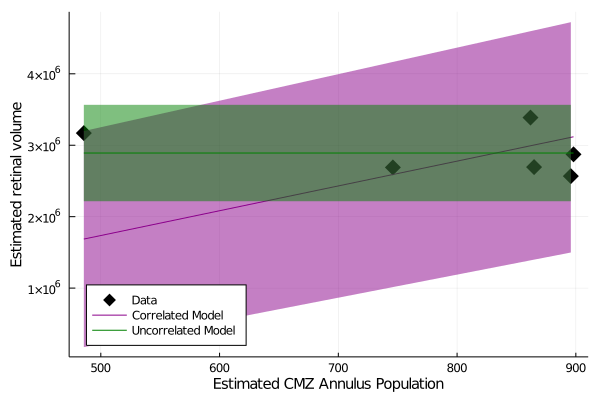
\includegraphics[width=.75\textwidth]{cmz/3dcorr.png}}    
    \caption{{\bf CMZ population and retinal volume estimates are uncorrelated at 3dpf}}
    Individual CMZ population estimate vs retinal volume estimate for 3dpf animals. Uncorrelated and correlated linear models of these variables are plotted as the mean$\pm$95\% CI of the predictive distribution of the fitted model.
    \label{gausscorrelation}
\end{figure}

From these analyses, we conclude that organismal variability in the CMZ population and retinal volume estimates are best described by independent Log-Normal distributions. Because Log-Normal distributions are simply transformed Normal Gaussian distributions, we may model our uncertainty about their parameters with Normal-Gamma distributions over the mean and variance of the underlying Normal distribution of the Log-Normal population model ("the underlying"). That is, our prior and posterior belief about the relative likelihood of values of the mean of the underlying may be modelled with a Normal distribution, and our beliefs about its variance with a Gamma, such that our joint uncertainty is the product of the two distributions. This is explained in more detail in \autoref{sec:NormalGamma}. A useful analytic feature of the Normal-Gamma prior is that the marginal posterior distribution of the mean, assuming an uninformative (ignorance) prior, is a location-scaled T distribution; this is so because the weighted sum of an infinite series of Normal distributions (i.e. the likelihood-weighted sum of all the Normal distributions that could underly the Log-Normal models), is a T distribution. T distributions are notably more resistent to outlier distortion than Normal distributions themselves are, and may be estimated with as few as two observations, making them highly flexible. Most of the descriptive statistics in the next section, therefore, calculate the credible interval for the posterior mean of the underlying by T distributions (with the correct change of variables by exponential transformation to produce the features of the correct Log-Normal distribution). Unfortunately, differences of T distributions are not, themselves, necessarily T-distributed, so we have relied on Monte Carlo estimation of rates of change of the these posterior means over time. With our Log-Normal models selected, and the descriptive tool of the posterior mean T distribution in hand, we turn now to a survey of the zebrafish CMZ in the first year of life.

\section{Survey of CMZ population and gross retinal contribution}

If it is true that the majority of zebrafish retinogenesis occurs postembryonically, and that models trained on embryonic data do not describe this period well, as seen in \autoref{chap:SMME}, what characterises this CMZ-driven phase of retinogenesis? We begin answering this question by presenting our estimates of individual CMZ annulus population and retinal volume over the first year of life, in \autoref{CMZoverall}, panels A and C.

\begin{figure}[!h]
    \makebox[\textwidth][c]{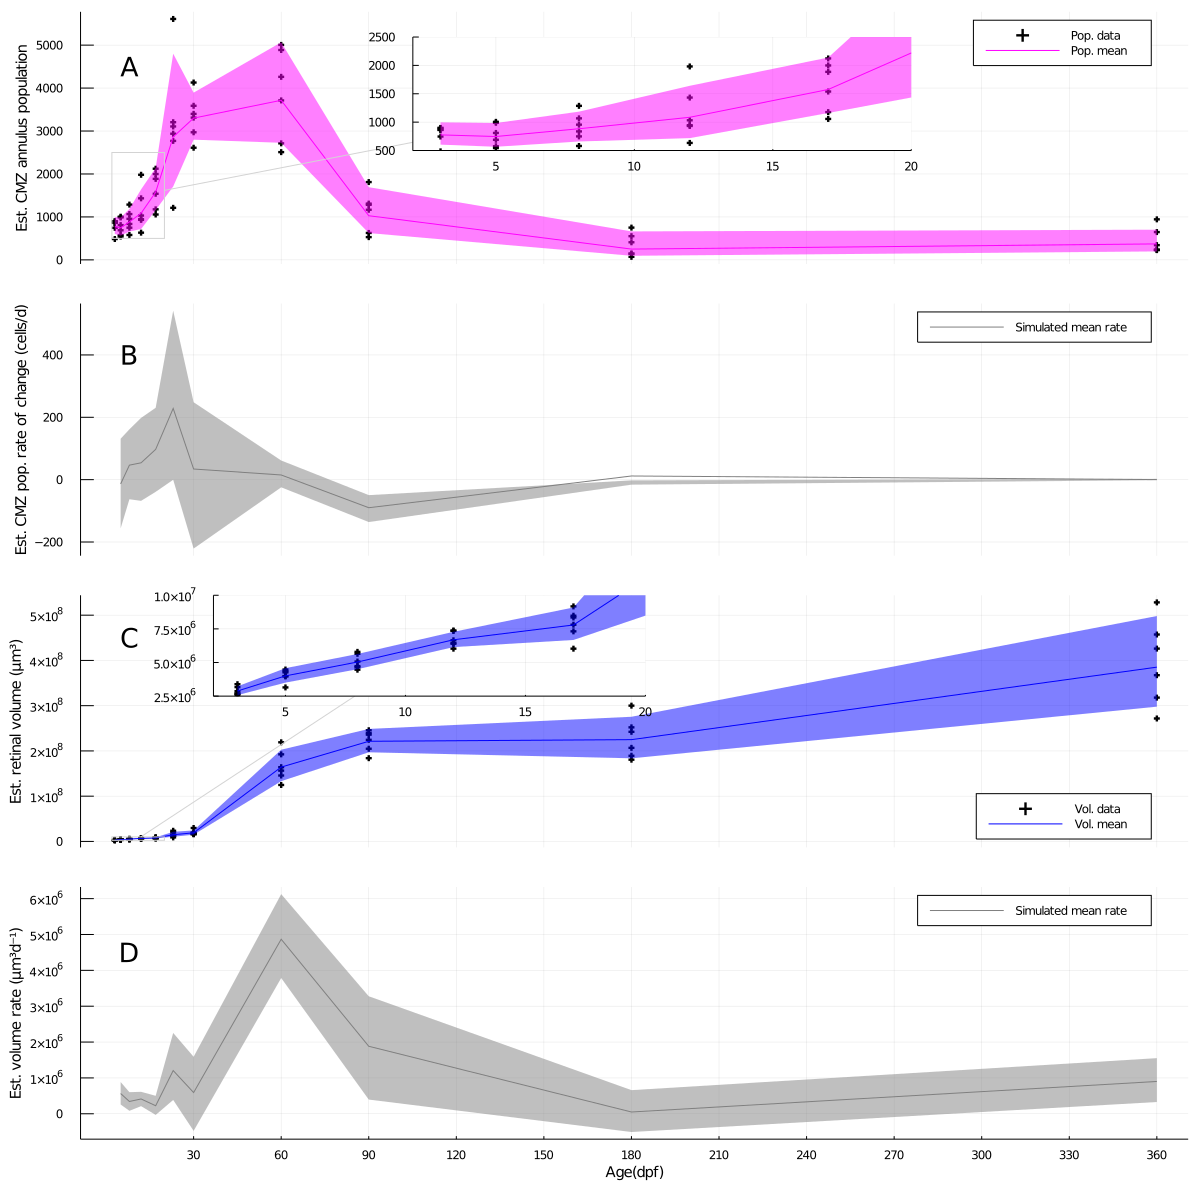
\includegraphics[width=1.\textwidth]{cmz/CMZoverall.png}}    
    \caption{{\bf Population and activity of the CMZ over the first year of \textit{D.rerio} life}}
    Panel A: Marginal posterior mean CMZ annulus population. Panel B: Marginal posterior mean retinal volume estimate. Insets in Panels A \& B display data from 3-17 dpf. Panel C: Marginal posterior mean of the proliferative index of the CMZ annulus, assayed by specified retinal neurons with incorporated thymidine from an 8hr pulse at the indicated ages. Panel D: Mean daily rate of volumetric increase of the neural retina, calculated as the difference in volumes between two ages over the number of elapsed days. All means are displayed in a band representing the $\pm 95 \%$ credible interval for the marginal posterior distribution of the mean.
    \label{CMZoverall}
\end{figure}

An initial, relatively quiescent period in the population history of the CMZ can be inferred from the lack of growth observed in the first week of life, as well as the observations in \autoref{rysCMZontogeny}, which demonstrate that CMZ RPCs are proliferating too slowly to be labelled by a day's pulse of a thymidine analogue at 5dpf in the wild-type and heterozygote siblings of npat mutants. Interestingly, we have good confidence that retinal volume continues to grow over this time; 99.56\% of the marginal posterior mass of the mean 5dpf estimate is above the 3dpf mean, suggesting that this proliferative pause is too short to appear in the retinal volume data.

In any case, the first two to three weeks of life (magnified in lens insets in panels A and C) appear to mark a relatively slow build in both estimated CMZ annulus population and retinal volume compared to the explosion which follows immediately thereafter. While zebrafish are better staged by size than age \cite{Parichy2009}, the onset of this explosive growth seems to come somewhat earlier than the typical metamorphic transition from larval to juvenile stages at ~45dpf \cite{Singleman2014}. This raises the question of the manner in which the CMZ contributes to the retina during the critical period of exponential growth of the organism, between about 45 and 90dpf. It is plausible, for instance, that the growth of the CMZ population mainly reflects the increased output of stem cells, with RPCs specifying at some steady rate, or that the CMZ builds itself up for a wave of niche exit and specification somewhat later, similarly to the sequence of events in the embryonic central retina.

In order to get a better sense of this timing, we simulated the mean daily rate of CMZ annulus population and retinal volume change, by performing Monte Carlo difference operations between samples from the marginal posterior means of subsequent timepoints. These simulated mean rates and their associated confidence intervals are plotted in \autoref{CMZoverall} panels B and D. These show the basic time-structure of the phenomenon; the large increase in simulated daily CMZ population growth rate occurs before the large increase in retinal volume, but the CMZ population estimate does not begin to drop off until 60dpf, by which time the majority of volumetric growth is complete. This seems to substantiate some combination of the scenarios outlined above: there is an early buildup of CMZ population around 18-30dpf, before CMZ RPCs begin to make their primary contribution to the retina between 30-60dpf, which is characterised by much slower population growth and more rapid volumetric growth, implying steady and elevated specification of RPCs. The greater uncertainty associated with our population estimates, relative to their magnitude, results in correspondingly less certainty about the size of the population growth rate spike. For instance, we calculate a >99\% probability that the mean retinal volumetric rate growth peak at 60 dpf is at least 6-fold greater than the mean at 30dpf. By contrast, only about 97\% of the posterior mean density of  the population growth rate at the 23d peak (230.2 $\frac{cells}{d}$) is greater than the mean at 3dpf, which is a small negative value (-5.5 $\frac{cells}{d}$). 

Subsequent to the bulk of the CMZ buildup and contribution to the retina, the population of the CMZ declines at about 39\% the rate of its peak ascent, with an estimated -90.1$\frac{cells}{d}$ by 90dpf. This process thins out the CMZ population to below its size immediately after embryogenesis, spread out over a much larger peripheral annulus, for a much less dense mature CMZ. Interestingly, the 95\% CI on the marginal posterior mean of estimated retinal volume at 180 dpf (ranging from \SI{1.84E8}{\cubic\micro\metre} to \SI{2.75E8}{\cubic\micro\metre}) completely encompasses the 95\% CI on volume at 90dpf (\SI{1.96E8}{\cubic\micro\metre}-\SI{2.48E8}{\cubic\micro\metre}), while the 360dpf mean (\SI{3.85E8}{\cubic\micro\metre}) is greater than six standard deviations from the 180dpf mean (\SI{2.25E8}{\cubic\micro\metre}). This suggests a possible second period of quiescence from approximately 90-180dpf, followed by steady contribution to the retina without a buildup in the CMZ population subsequently.

Given this rough description, it seems that the ontogeny of the CMZ as a stem cell niche could be well-described by different phases of activity, with different rates of proliferation and specification. It is not immediately clear what sort of periodization is justified by the data. It seems plausible that as few as two phases could explain the data well enough: an initial phase of logarithmic growth, with short cell cycle time and lower exit rate of RPCs from the CMZ into the specified neural retina, followed by a second phase of decay with longer cycle time and higher exit rate. On the other hand, perhaps some of the data features noted above justify a more bespoke model that captures, for instance, the initial quiescent period, or the post-180dpf growth of the retina. Because this is straightforwardly a question of how much model structure is justified by our data, we may address it as a model selection problem, using the system of Bayesian inference provided by nested sampling, and it is to this we now turn.

\section{Two-phase periodization of postembryonic CMZ activity by phased difference equation modelling}

To perform our model selection task, we wish to simulate the time-evolution of CMZ population and retinal volume. This requires us to supply initial values for the size of the simulated CMZ populations and the volumes of the simulated retinae they are associated with. Given the findings presented in \autoref{gausscorrelation}, we are justified in initializing CMZ population and retinal volume by independent samples from the Log-Normal models of their interindividual variability at 3dpf, at the end of embryogenesis and the beginning of CMZ-driven retinal growth. In order to produce new, simulated values of CMZ population and retinal volume, we apply a system of difference equations as follows, where $pop_n$ is the population at $n$ dpf, $CT$ is the mean cell cycle time of the population in hours, and $\epsilon$ is the proportion of the population at time $n-1$ that exits cycle and contributes to the volume of the specified neural retina, and $\mu_{cv}$ is the mean volume per cell contributed to the retina in \si{\cubic\micro\metre}:

\begin{equation}
    p_n=p_{n-1} \cdot 2^{\frac{24}{CT}} - p_{n-1} \cdot \epsilon
    \label{popeq}
\end{equation}

\begin{equation}
    v_n=v_{n-1} + p_{n-1} \cdot \epsilon \cdot \mu_{cv}
    \label{voleq}
\end{equation}

A model "phase" can then be defined by the $CT$ and $\epsilon$ parameters it applies to update the population and volume, over the appropriate number of days. The full parameterisation of a model with $p$ phases is given by $p$ pairs of $CT$ and $\epsilon$ values, $p-1$ phase transition times. $\mu_{cv}$, which is taken to apply equally to all phases, is estimated from 3 dpf nuclear measurements, as described in \autoref{sec:CMZestimates}. Given an initial population and volume sampled from the Log-Normal models of their interindividual distributions, \autoref{popeq} and \autoref{voleq} may be applied to these values difference equations can be applied to produce simulated sample values at the times actually observed. Many such samples obtained by Monte Carlo can be used to estimate Log-Normal distributions for the model parameters, which can be used to score the model against observations. By defining prior distributions over the model parameters, we may sample from the prior to initialize a model ensemble. The ensemble can then be compressed by nested sampling, moving each model-particle over the parameter space by Galilean Monte Carlo, as described in \autoref{GMC}. Using the typical procedures applied in nested sampling \cite{Skilling2006}, we estimated the Bayesian evidence, maximum a posteriori, and marginal posterior distributions on parameters for 2 and 3-phase models.

\begin{figure}[!h]
    \makebox[\textwidth][c]{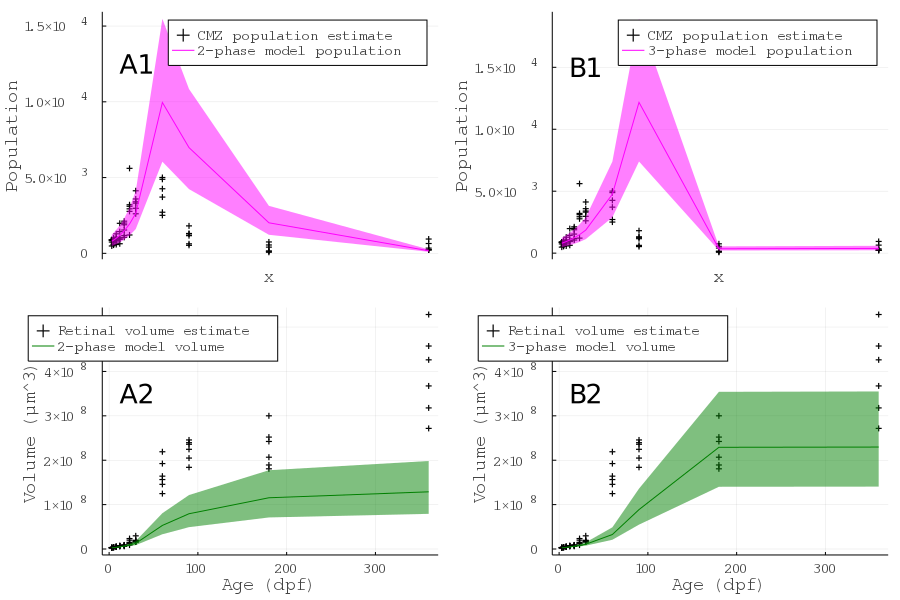
\includegraphics[width=1.2\textwidth]{cmz/a10pMAP.png}}    
    \caption{{\bf Maximum a posteriori output of periodization models}}
    \label{phaseMAPout}
    Population and volume estimates from observations (crosses) plotted with mean $\pm$ 95\% posterior mass model output, for the 2-phase model (A panels) and 3-phase model (B panels). A1,B1: population estimates. A2,B2: volume estimates. Insets provide magnified views of data from the first 30dpf.
\end{figure}

It is useful to begin with the maximum a posteriori model output, as this plainly shows the primary problem with this simple model; the model relationship between changes in CMZ population and changes in volume breaks down after 30dpf. That is, the later volume estimates are too large for the CMZ to produce, given the calculated cellular volume at 3dpf. The result is that the models fit the early population and volume data quite well, but the population peak is dragged upward and forward to produce more-likely volume output. While it is possible that the later CMZ contributes more volume per neuron to the cellular retina, it is much more likely that the volume approximation applies better to more-nearly spherical eyes at younger ages, than to the flattened eyes of later ages. Although we had hoped that the estimated retinal volume data would constrain the $\epsilon$ exit rate parameters, this was not the case, as discussed below. When we tried floating $\mu_{cv}$ as a variable within the model, the MAP results were similar (data not shown), suggesting that a constant value for $\mu_{cv}$ across ages is the problem in achieving good model fits, not the particular value chosen. This reinforces the idea that the problem relates to the breakdown of the retinal volume estimate at later ages.

While this limitation prevents either model from explaining the combined estimate datasets very well, they are in this sense under the same constraint, and so a reasonable inference about the number of phases justified by the data is still possible. Evidence estimates for the 2-phase and 3-phase models, given these data, are presented in \autoref{phasetable}. There are greater than 5600 orders of magnitude more evidence for the 2-phase model; this result has over 500 standard deviations of significance. This reflects the greatly expanded parameter space in the 3-phase model, which adds an additional 3 parameters to the 2-phase models' count of 5 parameters. The additional flexibility afforded by the 3rd phase in fitting the later volume data is unable to overcome the evidentiary penalty associated with the larger parameter space. We therefore conclude that, on the basis of these data, the 2-phase hypothesis must be accepted.

\begin{table}[!ht]
    \centering
    \caption{{\bf Evidence favours a 2-phase periodization of CMZ activity}}
    \begin{tabular}{|l|l|l|l|} \hline 
        {\bf 2-phase logZ} & {\bf 3-phase logZ} & {\bf logZR} & {\bf $\sigma$ Significance}\\ \hline
        {\bf -5583.1 $\pm$ 4.9} & -11247.0 $\pm$ 9.6 & 5664.0 $\pm$ 11.0 & 525.425\\ \hline 
    \end{tabular}
    \begin{flushleft} logZ: logarithm of p(D), the marginal likelihood of the data, or model evidence. logZR: evidence ratio; positive ratios in favour of the 2-phase model. Largest evidence value bolded.
    \end{flushleft}
    \label{phasetable}
\end{table}

While the parameter estimates associated with these models are clearly unreliable, they are useful to inspect in order to demonstrate some properties of nested sampling, and for comparison to the simulations to follow. To begin with, we present the parameterization of the MAP models displayed above in \autoref{phaseMAPtable}. Unsurprisingly, the selected 2-phase model begins with a first phase of rapid proliferation, with a $CT$ of 13.8 hr, followed by a second, slower phase of 27.2 hr. The imputed exit rate $\epsilon$ is greater than 200\% of the day's starting population in the first phase, suggesting that new cells exit the CMZ after about 12 hours, around one cycle, while the second phase exit rate is much less, with 86\% of the day's starting population exiting the CMZ, again suggesting a residency time of about one cycle. The imputed phase transition age is about 62dpf. Due to the volume estimate problem noted above, it is reasonable to believe that the $CT$ estimates are likely too short, the $\epsilon$ estimates too high, and the transition age too late; all favoured in order to produce higher volume estimates at later ages.

\begin{table}[!ht]
    \centering
    \caption{{\bf Maximum a posteriori parameter estimates for periodization models}}
    \begin{tabular}{|l|l|l|}
        \hline
        {\bf Parameter} & {\bf 2-phase MAP} & {\bf 3-phase MAP}\\ \hline
        Phase 1 $CT$ (h) & 13.8 & 14.3\\ \hline
        Phase 1 $\epsilon$ & 2.28 & 2.18\\ \hline
        Phase 2 $CT$ (h) & 27.2 & 35.4\\ \hline
        Phase 2 $\epsilon$ & 0.86 & 0.66\\ \hline
        Phase 3 $CT$ (h) & NA & 109.1\\ \hline
        Phase 3 $\epsilon$ & NA & 0.12\\ \hline
        Transition 1 age & 61.9 & 115.5\\ \hline
        Transition 2 age & NA & 252.1\\ \hline
        \end{tabular}
    \begin{flushleft}
    \end{flushleft}
    \label{phaseMAPtable}
\end{table}

Because nested sampling naturally produces samples from the posterior, we can estimate posterior distributions using the evidence values for these samples. We performed this by kernel density estimation, specifically to investigate the extent to which the marginal posterior distributions for the selected model are polymodal; that is, the extent to which the evidence supports multiple hypotheses about the parameters of the two imputed phases. Kernel density estimates (KDEs) for marginal posterior distributions on the 2-phase models' parameters are presented in \autoref{phasemarginals}. 

These estimates plainly reveal the polymodality of the posterior distributions, as well as the lack of constraint that the data impose on phase exit rates $\epsilon$. For instance, the first phase parameters (top left) display 3 major modes; the best evidentiated mode occurs between 15-20 hr $CT$, with the bulk of this posterior mass distributed above an exit rate of 1.0, but with a much larger range of $\epsilon$ supported than $CT$. The second phase parameters (bottom left) display even greater polymodality, with the bulk distributed around 140-150 hr $CT$, with an exit rate of less than .75. Plotting the two-dimensional marginal $CT$ from both phases (top right) reveals that these parameters are the best constrained by the data; still, the posterior is highly polymodal, with numerous combinations of $CT$ values receiving at least some support, although, obviously, shorter phase 1 $CT$ values combined with longer phase 2 $CT$ values are favoured. The marginal posterior distribution on the age at which the transition between phases occurs is plotted in the bottom right of \autoref{phasemarginals}; while the largest peaks of the KDE are at times greater than 50dpf, a substantial portion of the prior mass falls earlier than this, significant for the simulations to follow.

It should be noted here that the maximum a priori model parameters are not perfectly reflected in the KDE. While the $CT$ and $\epsilon$ parameters for both phases do fall broadly within the best-evidentiated posterior modes, they are not centered therein; moreover, the MAP phase transition time does not occur in the best-evidentiated transition time mode. As discussed in \autoref{sec:NS}, an important property of nested sampling is that the accuracy of evidence calculations is traded off against the accuracy of estimating the posterior distribution. Since we have here prioritized evidence estimation, this is the cause of this discrepancy; the MAP models themselves have relatively little weight in the KDE estimates.

\begin{figure}[!h]
    \makebox[\textwidth][c]{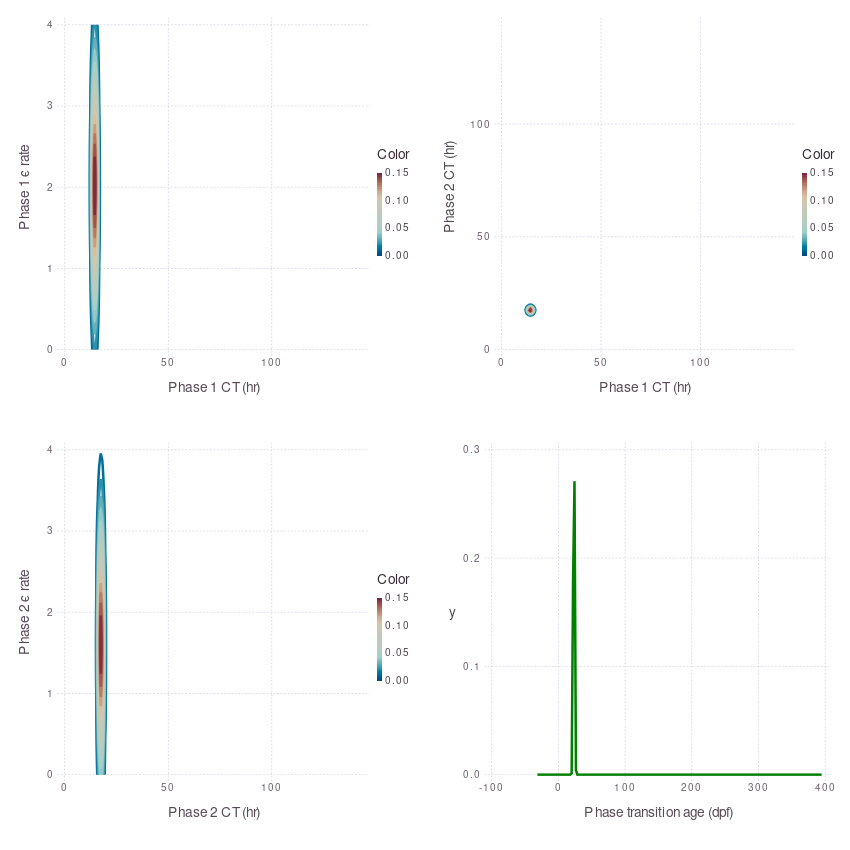
\includegraphics[width=1.\textwidth]{cmz/a10pmarginals.png}}    
    \caption{{\bf Kernel density estimates of marginal posterior parameter distributions, 2-phase model}}
    Line height (bottom right panels) or color (other panels) indicates the estimated marginal posterior mass present at the indicated parameter value.
    Top left panel: Phase 1 $\epsilon$ exit rate vs Phase 1 $CT$ cycle time (hr).
    Bottom left panel: Phase 2 $\epsilon$ exit rate vs Phase 2 $CT$ cycle time (hr).
    Top right panel: Phase 2 $CT$ cycle time (hr) vs Phase 1 $CT$ cycle time (hr).
    Bottom right panel: Estimated marginal posterior mass vs. phase transition age (dpf)
    \label{phasemarginals}
\end{figure}

We conclude that, while our global model of CMZ population and volumetric retinal contribution is too badly flawed to make credible parameter estimates, a 2-phase model of this activity is far better substantiated by the evidence than a 3-phase model. We proceed on this basis, accepting the 2-phase model, and taking up the idea of the "slice model" introduced in \autoref{ssec:slice}, to investigate modelling the CMZ RPC population more concretely, directly from sectional observations, rather than from the calculated population and retinal volume estimates presented above.

\section{Slice-model characterisation of asymmetrical CMZ population dynamics demonstrates anatomical homogeneity of proliferative schedule}
\label{sec:sliceGMC}

In the course of the preceding investigations, it became apparent that the population asymmetry mentioned in \autoref{chap:SMMEoutro} was not a static phenomenon, with the dorsal lobe of the CMZ annulus being consistently more populous than the ventral lobe, as generally implied by the sources covered in \autoref{chap:RPCreview}. Rather, both the extent and orientation of asymmetry seem to evolve over time. Sectional population totals for the dorsal and ventral CMZ are presented in \autoref{DVontology}, Panel A, alongside the related intra-individual asymmetry ratio in Panel B. The initially pronounced dorsal population and reduced ventral population both seem to go through the overall boom-bust progression of CMZ population, but their relative proportion within individuals reverses itself over the period from 17-90dpf. We also observed a similar phenomenon occurring across the naso-temporal axis over the same time period (\autoref{NTontology}).

\begin{figure}[!h]
    \makebox[\textwidth][c]{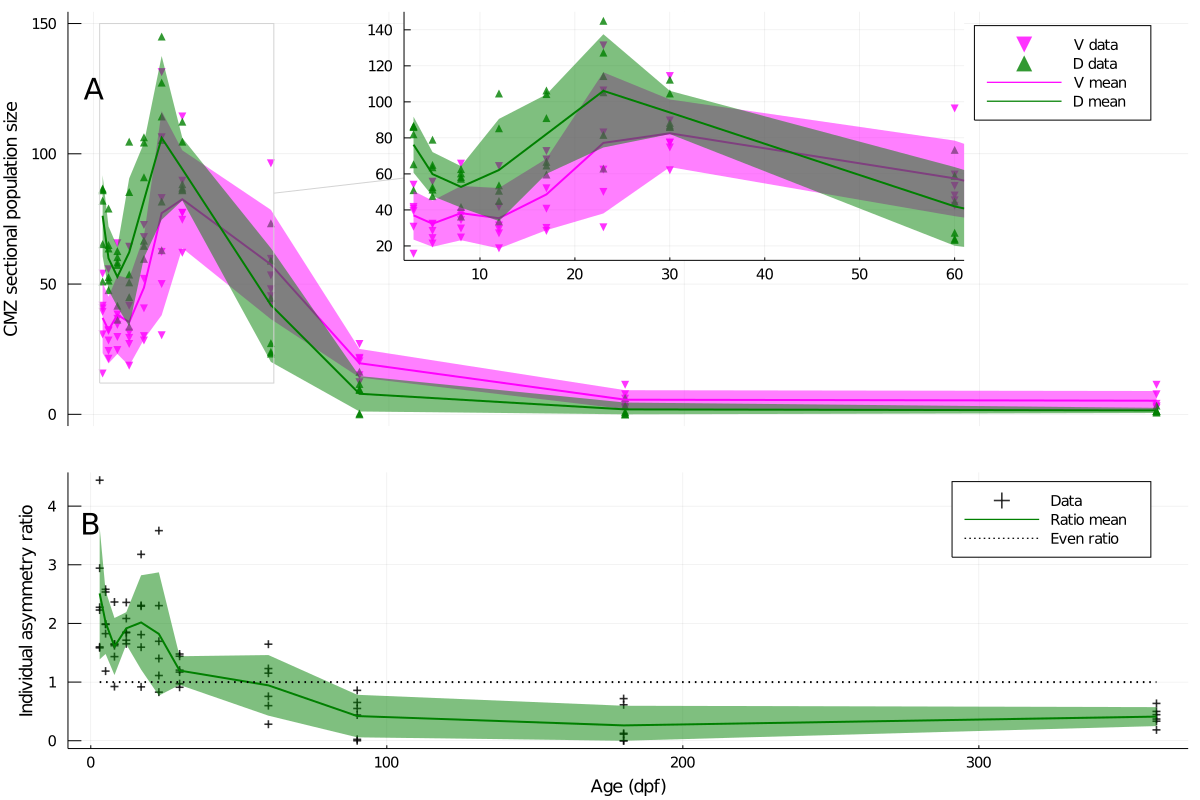
\includegraphics[width=1.2\textwidth]{cmz/DVontology.png}}    
    \caption{{\bf Developmental progression of dorso-ventral population asymmetry in the CMZ.}}
    Marginal posterior distribution of mean dorsal (D) and ventral (V) population size in 14$\mu$m coronal cryosections (panel A) or intra-individual D/V count asymmetry ratio (panel B), $\pm 95\%$ credible interval, n=5 animals per age. Data points represent mean counts from three central sections of an experimental animal's eye. 
    \label{DVontology}
\end{figure}

Inspected closely, these data provide a possible rationale for the reversal of asymmetry in the proliferative dynamics of the niche itself: the sectional (or ``slice'') population of the dorsal CMZ is increasing beyond its postembryonic minimum by 12dpf, while the ventral CMZ takes until 17dpf to exhibit a noticeable increase in size; moreover, the peak dorsal population is achieved by 23dpf, whilst ventrally the peak is only achieved at 30dpf. This strongly suggests that the dorsal and ventral CMZ populations undergo similar, time-shifted processes of proliferation from different starting populations. If this is so, an explanation for this time-shifted phenomenon could have fundamental relevance to predicting and controlling the proliferative behaviour of peripheral RPCs and stem cells.

To test this hypothesis, we used a ``slice model'' of the CMZ, where the thickness of the slice is taken to be the same as the observed cryosection thickness (\SI{14}{\micro\metre}). The population of the CMZ is modelled with a difference equation, as above, but with an additional exit term representing lateral, circumferential contributions of the CMZ to the generation of new, adjacent ``slices''. The value of this term is calculated from the difference in CMZ annulus diameter over the calculated time period implied by a power-law model of lens growth fitted to observations, as discussed in \autoref{sec:lenspopest}. The resultant difference equation is \autoref{sliceeq}. Terms are as defined above, except that $p_n$ is the sectional population at $n$ dpf, and not the total CMZ annulus population; additionally, $\eta$ is defined as the daily circumferential exit rate implied by the power-law model.

\begin{equation}
    p_n=p_{n-1} \cdot 2^{\frac{24}{CT}} - p_{n-1} \cdot \epsilon - \eta
    \label{sliceeq}
\end{equation}

We reasoned that, if the phase transition occurs earlier in the dorsal CMZ than in the ventral CMZ, there should be some informational gain in separating these observations vs. a combined total sum for both lobes of the slice annulus\footnote{The ``total'' model is required to supply double the circumferential exit rate of the dorsal or ventral models, to reflect the requirement for this ``full'' slice to grow both lobes of the eye}. In this case, the combination of two phase-shifted populations in the total model should produce a ``fuzzy'' peak relative to the separate modes. We therefore estimated the evidence, MAP, and posterior marginals for 2-phase models given the sectional sum, dorsal, and ventral populations. Given our belief that the whole-eye model presented above gives an over-long transition time, and in order to focus on the most informative subset of the data for our hypothesis, we restricted this analysis to the population data within the first three months of life.

The slice model proves to have much greater success at explaining sectional counts than the whole-eye model does at explaining the annulus population estimates; maximum a posteriori model output is presented in \autoref{dvMAPout}. In particular, all of the models adequately represent the early decline in sectional populations, arising from rapid early growth of the eye that exceeds the CMZs' proliferative capacity, without further ado; if there is not sufficient evidence to justify a separate, slow, late phase of proliferation, there is clearly none to justify a separate, slow, early phase. 

\begin{figure}[!h]
    \makebox[\textwidth][c]{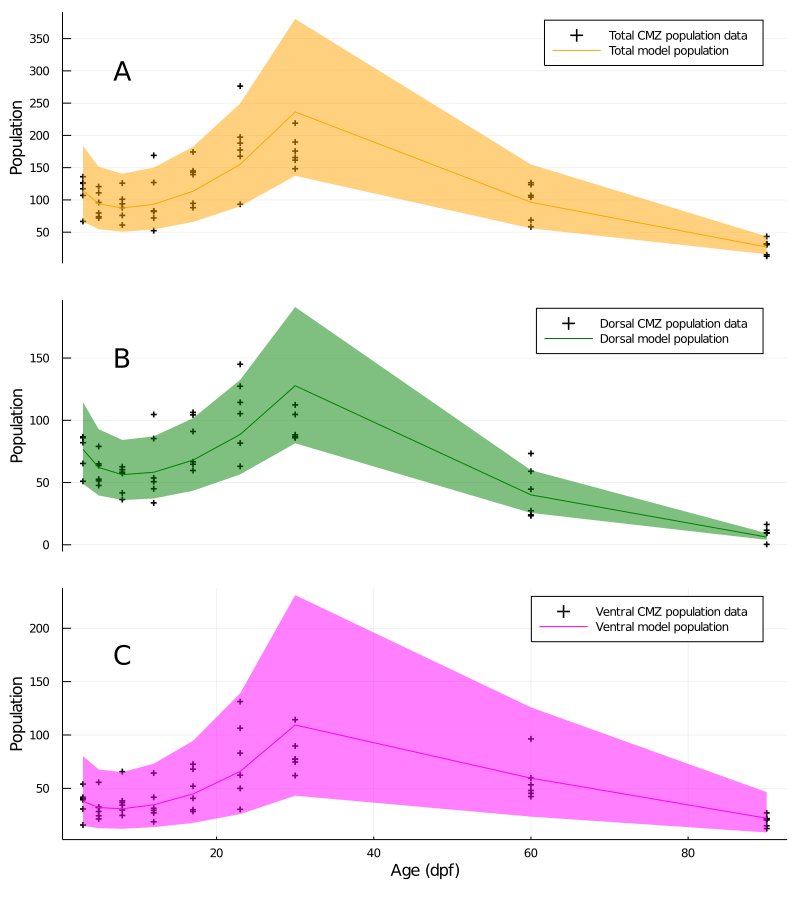
\includegraphics[width=.8\textwidth]{cmz/a10dvMAP.png}}    
    \caption{{\bf Maximum a posteriori output of total, dorsal, and ventral CMZ slice models}}
    \label{dvMAPout}
    Population and volume estimates from observations (crosses) plotted with mean $\pm$ 95\% posterior mass model output, for the total CMZ population model (panel A), dorsal CMZ population model (panel B), and ventral CMZ population model (panel C).
\end{figure}

The hypothesis that there is a time-shift in the phase transition across the dorso-ventral axis is thoroughly refuted by these models, in two ways. First, the evidence estimates demonstrate that we are not epistemically justified in separating the dorsal and ventral populations. The total-population slice model receives greater than 500 orders of magnitude more evidence than the joint evidence for the separate dorsal and ventral models, with greater than 190 standard deviations of significance, as displayed in \autoref{dvtable}. It is interesting to note that the evidence for the dorsal model is substantially lower than either the total or ventral models. This may indicate a causal influence on the dorsal population that is neither in the model nor acting on the ventral population, or it may be an uninteresting sampling effect. 

\begin{table}[!ht]
    \centering
    \caption{{\bf Evidence favours a combined slice model over separate dorsal and ventral models}}
    \begin{tabular}{|l|l|l|l|l|}
        \hline
        {\bf Total logZ} & {\bf Dorsal logZ} & {\bf Ventral logZ} & {\bf logZR} & {\bf $\sigma$ Significance}\\ \hline
        {\bf -498.1 $\pm$ 1.6} & -638.3 $\pm$ 1.8 & -371.7 $\pm$ 1.0 & 512.0 $\pm$ 2.6 & 194.861\\ \hline
        \end{tabular}
    \begin{flushleft} logZ: logarithm of p(D), the marginal likelihood of the data, or model evidence. logZR: evidence ratio; positive ratio in favour of the combined model. Largest evidence value bolded.
    \end{flushleft}
    \label{dvtable}
\end{table}

A second line of evidence indicating that this hypothesis is unsupported are the MAP model parameter values, summarized in \autoref{dvMAPtable}. The MAP phase transition age for the total slice model is functionally identical\footnote{That is, both values round to 35 days in the likelihood function, which uses the discrete difference equation, with a step size of 1dpf, as indicated above.} to that for the ventral model, and within two days of the MAP transition for the dorsal model. Additionally, the dorsal MAP transition is actually later than the ventral date, which further suggests the original model-idea of a time-shifted late ventral phase change is unsupported by evidence. Reassuringly, the MAP parameters for the total slice model are similar to those found for the 2-phase MAP in \autoref{phasemarginals}. Interestingly, the MAP phase parameters differ markedly between the split dorsal\/ventral models and the total slice model, although all suggest a longer $CT$ and lower $\epsilon$ for the second phase. This observation suggests that the additional noise incurred from splitting the sectional CMZ population into dorsal and ventral lobes has a strong effect on parameter estimates. This may provide a practical reason to prefer combining these counts in slice models, beyond the fact that it is epistemically unjustified on the support of these data. 

\begin{table}[!ht]
    \centering
    \caption{{\bf Maximum a posteriori parameter estimates for slice models}}
    \begin{tabular}{|l|l|l|l|}
        \hline
        {\bf Parameter} & {\bf Total MAP} & {\bf Dorsal MAP} & {\bf Ventral MAP}\\ \hline
        Phase 1 $CT$ (h) & 16.1 & 29.1 & 20.5\\ \hline
        Phase 1 $\epsilon$ & 1.72 & 0.69 & 1.15\\ \hline
        Phase 2 $CT$ (h) & 23.5 & 37.0 & 55.2\\ \hline
        Phase 2 $\epsilon$ & 1.06 & 0.62 & 0.38\\ \hline
        Transition age & 35.5 & 37.2 & 35.8\\ \hline
        \end{tabular}
    \begin{flushleft} 
    \end{flushleft}
    \label{dvMAPtable}
\end{table}

Examining the marginal posterior distributions of the total slice model, presented in \autoref{dvmarginals}, shows that exit rate posteriors are no less constrained than the whole-eye model, suggesting the retinal volume estimate supplies little additional  information, beyond the population estimate, regarding the rate at which RPCs leave the niche. However, the marginal posteriors on cycle length are less constrained than the whole-eye model, with noticeably less separation between modes, which suggests that the volume estimate may nonetheless narrow the range of credible $CT$ values. This suggests a rationale for pursuing better volumetric estimates for retinae from fish older than 30 dpf. The posterior distribution on the age of phase transition indicates that many values for this parameter retain some credibility, and, like the whole-eye model marginals in \autoref{phasemarginals}, the MAP estimate does not occupy the most probable KDE kernel for this value, for the same reason noted above.

\begin{figure}[!h]
    \makebox[\textwidth][c]{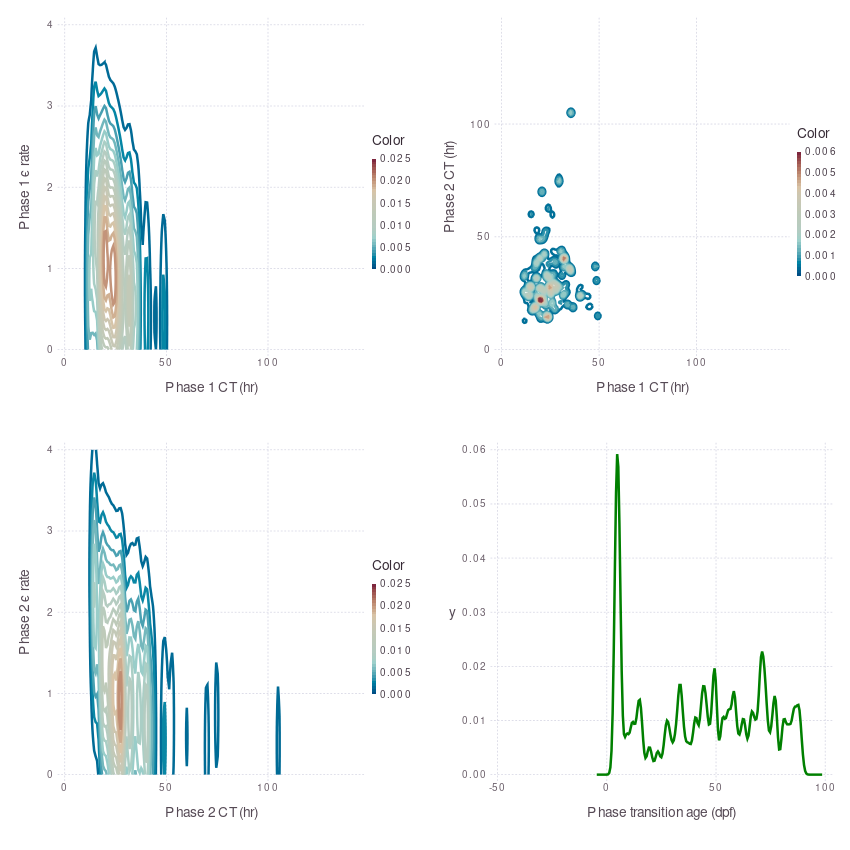
\includegraphics[width=1.\textwidth]{cmz/a10dvmarginals.png}}    
    \caption{{\bf Kernel density estimates of marginal posterior parameter distributions, total slice model}}
    Line height (bottom right panels) or color (other panels) indicates the estimated marginal posterior mass present at the indicated parameter value.
    Top left panel: Phase 1 $\epsilon$ exit rate vs Phase 1 $CT$ cycle time (hr).
    Bottom left panel: Phase 2 $\epsilon$ exit rate vs Phase 2 $CT$ cycle time (hr).
    Top right panel: Phase 2 $CT$ cycle time (hr) vs Phase 1 $CT$ cycle time (hr).
    Bottom right panel: Estimated marginal posterior mass vs. phase transition age (dpf)
    \label{dvmarginals}
\end{figure}

On the basis of this analysis, the best available hypothesis about the observed ontogeny of RPC population asymmetry across the dorsoventral axis is the pre-establishment of differential population size by asymmetrical progress of the embryonic specification wave, rather than differential proliferative schedules.

\subsection{Cumulative thymidine labelling supports Galilean Monte Carlo Nested Sampling parameter estimate}

The similarity of $CT$ and $\epsilon$ exit rate parameters in the whole-eye and total slice models, despite the defective cellular retinal volume estimate, suggests that these values may be relatively accurate. In order to partially validate this idea, we examined 3dpf CMZ RPCs labelled with a 10.5 hour pulse of the thymidine analogue EdU. We used the Empirical Bayes approach to estimate the evidence for separate Nowakowski-style \cite{Nowakowski1989} linear models for the dorsal and ventral CMZ, against a model for both subpopulations combined. While this model is inadequate for reasons described in \autoref{sec:Nowakowski}, it can serve to substantiate the first phase cycle time parameter. These results are summarized in \autoref{cumEdUtable}, with the relevant linear regressions displayed in Supplementary \autoref{cumEdUlinreg}.

\begin{table}[!ht]
    \centering
    \caption{{\bf Evidence favours whole-CMZ linear cycle models over separate D/V models}}
    \begin{tabular}{|l|l|l|l|} 
        \hline {\bf Model} & {\bf Implied $T_c$ (hr)} & {\bf Implied $T_s$ (hr)} & {\bf logZ}\\ \hline 
        Dorsal & 14.7 $\pm$ 1.6 & 1.38 $\pm$ 0.76 & 7.778\\ \hline 
        Ventral & 14.0 $\pm$ 1.2 & 0.8 $\pm$ 0.58 & 15.202\\ \hline
        Combined & 14.6 $\pm$ 1.1 & 1.25 $\pm$ 0.53 & {\bf26.165}\\ \hline
    \end{tabular}
   
    \begin{flushleft} $T_c$: calculated cell cycle time. $T_s$: calculated s-phase length. logZ: logarithm of p(D), the marginal likelihood of the data, or model evidence.  Largest evidence value bolded.
    \end{flushleft}
    \label{cumEdUtable}
\end{table}

Firstly, there are approximately 3 orders of magnitude of evidence in favour of the combined model vs. the joint evidence for separate models (ie. 26.165 vs. 22.980). There is no evidence, on this basis, for differing cell cycle characteristics across the D/V retinal axis of asymmetry at 3dpf. Moreover, the Nowakowski-calculated cell cycle time $T_c$ for the combined model, 14.6 $\pm$ 1.1 hr, includes the whole-eye MAP first phase $TC$, 13.8 hr, within one standard deviation, while the total slice-model first phase $TC$, 16.1, is within two. This confirms that the differing D/V MAP parameter estimates observed in the slice model are unsubstantiated; the evidence supports broadly similar cell cycle characteristics across anatomical axes in 3dpf CMZ RPCs. Moreover, at least the MAP cell cycle times implied by our model selection time seem realistic, given the assumptions of the of Nowakowski model. That said, the data clearly diverge from a linear trend toward the end of the pulse, and the calculated S phase lengths are unrealistically short, showing the limitations of this model.

\section{The CMZ contributes stably to each cellular layer with time-variable lineage composition}

By labelling CMZ RPCs with the thymidine analogue EdU in an 8 hour pulse at 3, 23, and 90 dpf, followed by histochemical analysis for known zebrafish retinal neural lineage markers after a 7 day chase, we investigated the possibility that RPC lineage outcomes change over the life of the organism. This hypothesis is of particular interest, as differences in the mosaic organisation of embryonically-contributed central retina and CMZ-contributed peripheral retina remain unexplained \cite{Allison2010}. It may, moreover, have clinical significance, were quiescent peripheral stem cells to be entrained for regnerative medical purposes, as their lineage outcomes are may be different than embryonic RPCs.  We used antibodies raised against Pax6 and Isl2b to mark retinal ganglion cells (RGCs) of the ganglion cell layer and amacrine cells of the inner nuclear layer. Anti-glutamine synthetase (GS) and anti-PKC$\beta$ were used to mark M\"{u}ller glia (MG) and bipolar cell (BPC) populations of the INL. The unique flattened nuclear morphology of horizontal neurons was used to identify them. Lastly, the antibody Zpr1, directed against an unknown antigen present in photoreceptors with double cone morphology, was used to mark these cells.

\begin{figure}[!h]
    \makebox[\textwidth][c]{\includegraphics[width=1.2\textwidth]{cmz/lineage.png}}    
    \caption{{\bf Representative 23dpf lineage marker confocal micrographs}}
    Panel A1: RGC/Amacrine staining group. A2: Isl2b channel. A3: Pax6 channel.

    Panel B1: MG/BPC staining group. B2: PKC$\beta$ channel. B3: GS channel.

    Panel C: Double cone staining group. Zpr1 channel.

    GCL: Ganglion cell layer. INL: Inner nuclear layer. ONL: Outer nuclear layer.
    \label{staininggroups}
\end{figure}

Observations were collected in "staining groups", which combined histological markers; representative confocal micrographs from this study in animals pulsed at 23dpf are displayed in \autoref{staininggroups}, while data from all ages are plotted in \autoref{layercontributions}. It is worth noting that the relative position of the CMZ-contributed cohort is very different in older animals, with 7 days of chase time being just enough for the majority of the 90dpf cohort to be reliably located within the specified neural retina, as depicted in supplementary \autoref{90dpfcohort}. Because we suspect that CMZ-contributed retinal cohorts may be subject to a process of attrition, and that this turnover might be higher near the CMZ, as discussed in \autoref{sec:neuralfate}, if this hypothetical turnover process has differential effects over time on specified retinal neurons of different lineages, results may not be directly comparable between ages. With that caveat, we proceed to the lineage data.

\begin{figure}[!h]
    \makebox[\textwidth][c]{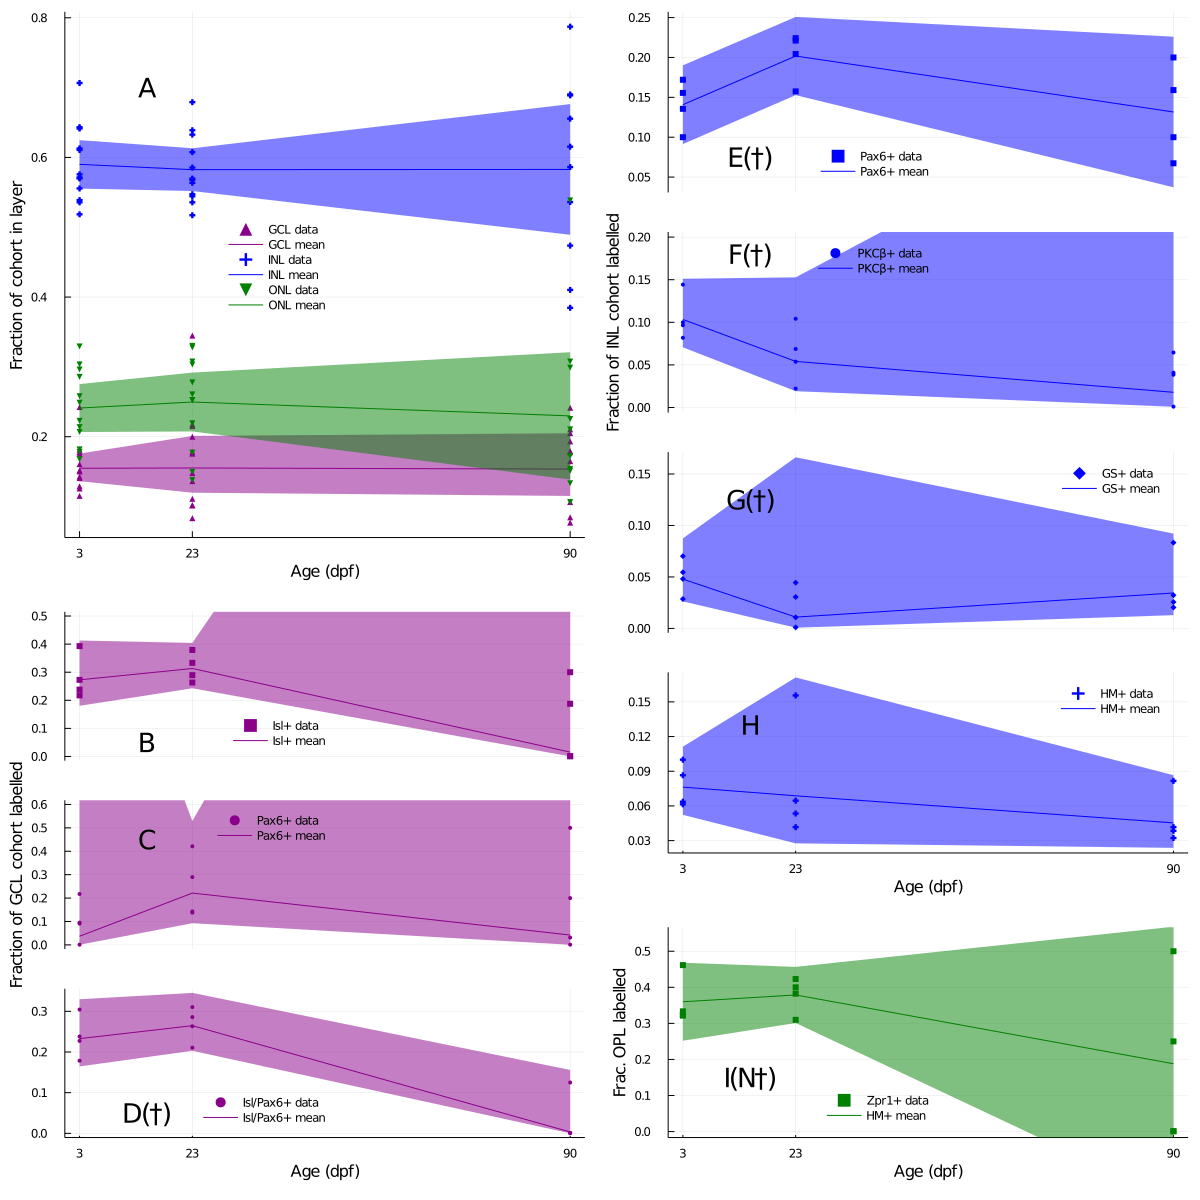
\includegraphics[width=1.2\textwidth]{cmz/layercontributions.png}}    
    \caption{{\bf Second-phase declines in CMZ-contributed Isl\/Pax6+ RGCs, PKC$\beta$+ bipolar neurons, and Zpr1+ double cones}}
    Overall fraction of CMZ-contributed cohort entering cellular layers (Panel A), or fraction of the layer subcohort expressing the noted immunohistochemical marker of lineage. All mean values are presented as marginal posterior means $\pm$ 95\%CI.

    $\lambda$: Fractional lineage contribution is modelled Log-Normally

    $\dagger$: Evidence supports time-varying model of fractional lineage contribution

    Magenta: GCL measurements; Blue: INL measurements; Green: ONL measurements
    \label{layercontributions}
\end{figure}

These data take the form of fractions of the presumptive CMZ-contributed, thymidine-labelled cohort entering each of the three cellular layers (panel A of \autoref{layercontributions}), or the subfraction of the cohort within a given layer expressing a particular cellular marker (Panels B-I). While some variability is apparent in all of the measurements, it is unclear whether it is well-described as time-dependent in most cases. In order to address the question of whether CMZ layer or lineage outcomes differ over time, we needed to assess the joint evidence for separate models of each measurement at each age, against the evidence for a single model of the measurement for all of the assessed ages. 

Because it is not immediately obvious that these fractional measurements are better described Log-Normally as the underlying population counts are, we first assessed the joint evidence for Normal and Log-Normal models of the data, summarized in Supplementary \autoref{lineage_nlnev}. Our evidence supports Normal modelling of all measurements aside from GCL Pax6-\footnote{Measured Pax6-positive fractional lineage contributions to the INL support Normal models better than Log-Normal.}, PKC$\beta$-, GS-, and Zpr1-positive cells, along with those displaying horizontal nuclear morphology. We noted that the evidence estimates contradicted simple likelihood ratio tests in most cases, as summarized in Supplementary \autoref{lineage_lhratio}, with only GCL Pax6+, GS+, and HM+ results in agreement with the evidence estimates. This demonstrates a case where full evidence estimation produces the opposite result from maximum likelihood methods for multiple measurements.  Without a clear fundamental justification for uniformly preferring one model or the other, we selected the best-supported model for each measurement. We estimated the evidence for an age-marginalized model, representing stable contribution to the layer or lineage over time, and compared this to the joint evidence for separate models at each age, representing a time-varying contribution model. These estimates are presented in \autoref{lineage_ev}.

\begin{table}[!ht]
    \caption{{\bf Evidence supports stable layer contributions with time-varying lineage contributions}}
    \begin{tabular}{|l|l|l|l|l|l|l|} 
        \hline
        {\bf Layer} & {\bf Marker} & {\bf Cell type} & {\bf Stable logZ} & {\bf Time-vary logZ} & {\bf logZR} & {\bf $\sigma$ sign.}\\ \hline \hline
        GCL & Cohort & All GCL cells & {\bf -41.64 ± 0.63} & -57.84 ± 0.34 & 16.2 ± 0.72 & 22.5\\ \hline \hline
        GCL & Isl2b & RGC & {\bf -47.58 ± 0.84} & -65.6 ± 0.93 & 18.0 ± 1.3 & 14.4\\ \hline
        GCL & Pax6 & Displaced am. & {\bf -32.65 ± 0.68} & -42.5 ± 1.3 & 9.9 ± 1.5 & 6.6\\ \hline
        GCL & Isl2b/Pax6 & RGC subtype & -40.94 ± 0.77 & {\bf -10.53 ± 0.26} & -30.41 ± 0.81 & 37.5\\ \hline \hline
        INL & Cohort & All INL cells & -83.5 ± 1.0 & {\bf -72.97 ± 0.83} & -10.5 ± 1.3 & 8.0\\ \hline \hline
        INL & Pax6 & Amacrine cell & {\bf -32.65 ± 0.68} & -42.5 ± 1.3 & 9.9 ± 1.5 & 6.6\\ \hline
        INL & PKC$\beta$ & Bipolar cell & -10.52 ± 0.46 & {\bf 4.61 ± 0.49} & -15.13 ± 0.68 & 22.4\\ \hline
        INL & GS & M\"{u}ller glia & {\bf 13.69 ± 0.36} & 3.98 ± 0.7 & 9.7 ± 0.79 & 12.3\\ \hline
        INL & HM & Horizontal cell & {\bf 9.81 ± 0.37} & -1.18 ± 0.67 & 10.99 ± 0.77 & 14.3\\ \hline \hline
        ONL & Cohort & All ONL cells & {\bf -73.06 ± 0.84} & -116.56 ± 0.88 & 43.5 ± 1.2 & 35.7\\\hline \hline
        ONL & Zpr1 & Double cones &  -41.17 ± 0.75 & {\bf -29.28 ± 0.54} & -11.89 ± 0.92 & 12.9\\  \hline
    \end{tabular}
   
    \begin{flushleft}logZ: logarithm of p(D), the marginal likelihood of the data, or model evidence.  Largest evidence values bolded. logZR: evidence ratio; positive values in favour of stable model.
    \end{flushleft}
    \label{lineage_ev}
\end{table}

These calculations speak to overall layer-stability of retinal contributions across this period, with strong evidence for a time-varying model for particular lineages. In particular, we determined that time-varying models of Isl/Pax6+ cells in the GCL, PKC$\beta$+ bipolar cells in the INL, and Zpr1+ double cones of the ONL are all well-supported, with more than 8 standard deviations of significance in each case. Interestingly, the trend of the posterior mean for all three of these lineages declines from the early postembryonic period (3dpf) to the late juvenile period (90dpf). It is tempting to speculate that these lineages may be functionally related; however, we have no specific evidence that would implicate Isl2b/Pax6 double-positive RGCs in circuits with bipolar cells or double cones. Still, this provides a plausible explanation for the observation of a more-ordered retinal mosaic in later retinal contributions relative to the embryonic central remnant: if one or more sublineages in each layer is depleted in older fish, this would result in a different overall mosaic pattern through the layer-structure as the neurons associate and pack together. Based on the overall timing of these changes, we tentatively ascribe this differential lineage production to the second phase of CMZ contribution in our periodisation; the data do not provide enough information to test evidence for testing timing hypotheses with more precision.

Lastly, we investigated the possibility that there might be detectable differences in layer or lineage contributions across the dorso-ventral axis; we tested this by measuring the evidence for age-marginalized combined models of fractional contribution against age-marginalized models split along the dorso-ventral axis. We found no evidence to support this hypothesis. These results are presented in Summary \autoref{lineage_dvev}.

\FloatBarrier

\section{Early retinal cohorts of the \textit{D. rerio} retina are turned over at a low rate by 4C4-positive microglia}
\label{sec:neuralfate}
Recently, extensive neural death has been reported in older zebrafish retinae, described as a "neurodegenerative pathology" and suggested as a model of age-related neurodegeneration \cite{Vanhoucke2018}. In the course of our thymidine analogue pulse-chase studies, we noted that it often appeared that CMZ-contributed cohorts were less numerous noticeably only a month or two after their entry into the neural retina, even in juveniles of 30-90 days of age. Moreover, we observed numerous 4C4-positive microglia associating with the CMZ, as displayed in Supplementary \autoref{4C4overview}, which raised the possiblity that these cells may be involved in pruning CMZ contributions. If neural retinal turnover is a general phenomenon throughout the life of the organism, this has fundamental implications for the view that this phenomenon should be treated as pathological, rather than constitutive. However, the thinning phenomenon could be explained by processes involved in the changing morphology and geometry of the neural retina during this period. In particular, the neural retina thickens noticeably over this time period, as displayed in Supplementary \autoref{morphology}. Although this increase is due in large part to the lengthening of photoreceptor outer segments, the inner nuclear layer is also significantly thickened. It is plausible that this process involves a compaction of the neurons along the coronal axis typically sampled, thus appearing to lose cells over time without this actually occurring. 

In order to investigate this phenomenon, we administered 24 hr pulses of EdU to 1dpf embryos, and followed with 24 hr pulses of BrdU at 23dpf to mark a CMZ-contributed cohort near the height of its activity. By taking both coronal and transverse sections through animals at 30, 60, and 90 dpf, we sampled these cohorts from both morphological axes of the retina and counted labelled sectional totals. Data from the axes were combined to account for the possibility of the cohorts being compacted on the coronal plane and extended on the transverse one. In order to test the hypothesis of early turnover, we estimated the evidence for linearly correlated and uncorrelated models of cohort population over time, using the \hyperref[empiricalBayes]{Empirical Bayes} regression method. In effect, we suppose that if the addition of a time-dependent term in the correlated regression model is justified by the evidence at these early ages, this supplies some support to the notion that \textit{D. rerio} retinal turnover is a lifelong phenomenon; if not, the apparent contraction of the cohorts is likely a function of one or more of the alternative morphological explanations noted above, or is occurring at too low a rate to be detected by these means. The results are summarized in \autoref{turnovertable}, with the regressions plotted in Supplementary \autoref{a27linreg}.

\begin{table}[!ht]
    \centering
    \caption{{\bf Evidence for linear regression models supports early cohort population stability}}
    \begin{tabular}{|l|l|l|l|}
    \hline
    {\bf Measurement} & {\bf Stable logZ} & {\bf Declining logZ} & {\bf logZR}\\ \hline
    1dpf Central Remnant & {\bf -212.953} & -214.167 & 1.213\\ \hline    
    30dpf Cohort & {\bf -107.567} & -110.827 & 3.261\\ \hline
    \end{tabular}
   
    \begin{flushleft}logZ: logarithm of p(D), the marginal likelihood of the data, or model evidence.  Largest evidence values bolded. logZR: evidence ratio; positive values in favour of stable model.
    \end{flushleft}
    \label{turnovertable}
\end{table}

In both cases, there is better evidence for a model of cohort population that is stable over time than one correlated with time, indicating that the additional model complexity implied by allowing turnover is unjustified for this early period. Despite this, we did find isolated instances where members of these cohorts were visibly being engulfed by 4C4-positive microglia; one such event is depicted in \autoref{4C4micrograph}. This indicates that some level of turnover is indeed occuring during this time. The evidence ratio in favour of the uncorrelated models is not overwhelming, which suggests that the best interpretation of the data is that the cohorts are not turned over at a high enough rate to be detectable in the early period, although the process does occur even at this early age. In order to determine whether expending additional computational effort to supplement an Emprical Bayes linear regression with GMC-NS evidence estimation, we followed on with estimating the evidence for age-marginalized Log-Normal models of the population counts against age-differentiated models, representing time-constant and time-varying population models. This investigation proves to resolve any ambiguity: no time-varying model is justified by the available evidence, as summarized in \autoref{turnoverGMCtable}

\begin{figure}[!h]
    \makebox[\textwidth][c]{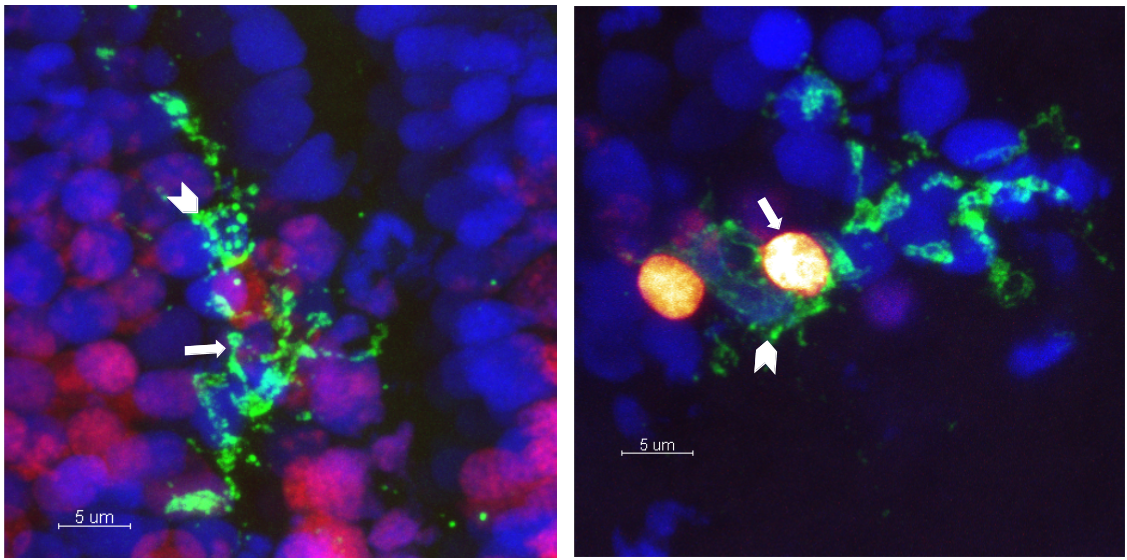
\includegraphics[width=1.\textwidth]{cmz/4C4engulfment.png}}    
    \caption{{\bf 4C4+ microglia associate with and engulf EdU-labelled CMZ contributions in the specified neural retina}}
    Representative maximum intensity projections from confocal micrographs of 14\si{\micro\metre} coronal cryosections through 30dpf zebrafish eyes labelled at 23dpf with EdU.
    
    Blue: Hoechst 33258 nuclear counterstain. Green: Microglia labelled with 4C4 antibody. Red-orange-yellow: Intensity scale of EdU staining, indicating cellular origin in the 23dpf CMZ.

    Chevrons: microglial nuclei. Arrows: EdU-positive nuclei found within 4C4-labelled extent of microglial cell body and appendages.
    \label{4C4micrograph}
\end{figure}

\begin{table}[!ht]
    \centering
    \caption{{\bf GMC-NS evidence estimates confirm Empircal Bayes analysis of early cohort stability}}
    \begin{tabular}{|l|l|l|l|l|} \hline 
        {\bf Cohort} & {\bf Time-constant logZ} & {\bf Time-varying logZ} & {\bf logZR} & {\bf $\sigma$ Significance}\\ \hline
        Embryonic central remnant & {\bf -314.6 ± 3.6} & -413.4 ± 5.1 & 98.8 ± 6.2 & 15.8\\ \hline
        1 month CMZ & {\bf -312.3 ± 5.9} & -416.6 ± 4.5 & 104.3 ± 7.4 & 14.1\\ \hline
    \end{tabular}
    \begin{flushleft} logZ: logarithm of p(D), the marginal likelihood of the data, or model evidence. logZR: evidence ratio; positive ratios in favour of the 2-phase model. Largest evidence value bolded.
    \end{flushleft}
    \label{turnoverGMCtable}
\end{table}

\section{Summary: Two-phase periodisation of postembryonic CMZ activity \& functional significance of CMZ activity}
We have established that our data is best explained by a 2-phase periodization of postembryonic CMZ activity, with an initial month-long phase of relatively rapid proliferation and lower rate of exit into the specified neural retina, followed by a second phase of slower proliferation and higher exit rate. We have established posterior distributions on likely parameter ranges that convey the uncertainty we have about them; these demonstrate that our estimates of cell cycle lengths are much more certain than of exit rates.  The population of the CMZ displays an asymmetric structure which reverses over time; we have demonstrated that this is not due to time-shifting of the two proliferative phases across anatomical axes, but rather seems to be arise from a difference in the relative rates of exit from the proliferative population into the specified neural retina. The proportional composition of CMZ-driven contributions is highly stable over this time, and does not display variability over the dorso-ventral axis. We found evidence for one exception to this pattern: the relative proportion of PKC$\beta$-positive bipolar cells found in CMZ-generated cohorts declines over the first three months of life. Finally, we have shown that microglia-mediated turnover of retinal neurons is occurring at a rate too low to have a measurable effect on cohort sizes during this time.

We are interested in identifying macromolecular factors involved in the control of proliferation and specification of CMZ RPCs. These analyses suggest that these may be most profitably investigated at different ages. If we take the phase transition times estimated in \autoref{sec:sliceGMC} to be the most reliable in this chapter, this would suggest that factors implicated in proliferative control would be best identified by assays bracketing the transition time at ~35dpf; we would expect the rate of change of macromolecular correlates of cycle activity to be greatest around this time. There seems to be little spatial structure apparent in proliferative activity, and it is probably pointless to break out these data by anatomical location. By contrast, it would be best to investigate factors involved in specification by contrasting their parameters across anatomical axes at early postembryonic (~3dpf) and early adult (~90dpf) ages, when the apparent asymmetry in niche exit rates is most pronounced. Moreover, since this asymmetry reverses itself over this time, this provides a natural means to establish correlates that are likely causally related to regulating the process of specification and niche exit, since these should be enhanced dorsally in the early ages and ventrally at later ages.

%\section{Toward cell-based computational models of the CMZ}